% Options for packages loaded elsewhere
\PassOptionsToPackage{unicode}{hyperref}
\PassOptionsToPackage{hyphens}{url}
%
\documentclass[
]{article}
\usepackage{amsmath,amssymb}
\usepackage{iftex}
\ifPDFTeX
  \usepackage[T1]{fontenc}
  \usepackage[utf8]{inputenc}
  \usepackage{textcomp} % provide euro and other symbols
\else % if luatex or xetex
  \usepackage{unicode-math} % this also loads fontspec
  \defaultfontfeatures{Scale=MatchLowercase}
  \defaultfontfeatures[\rmfamily]{Ligatures=TeX,Scale=1}
\fi
\usepackage{lmodern}
\ifPDFTeX\else
  % xetex/luatex font selection
\fi
% Use upquote if available, for straight quotes in verbatim environments
\IfFileExists{upquote.sty}{\usepackage{upquote}}{}
\IfFileExists{microtype.sty}{% use microtype if available
  \usepackage[]{microtype}
  \UseMicrotypeSet[protrusion]{basicmath} % disable protrusion for tt fonts
}{}
\makeatletter
\@ifundefined{KOMAClassName}{% if non-KOMA class
  \IfFileExists{parskip.sty}{%
    \usepackage{parskip}
  }{% else
    \setlength{\parindent}{0pt}
    \setlength{\parskip}{6pt plus 2pt minus 1pt}}
}{% if KOMA class
  \KOMAoptions{parskip=half}}
\makeatother
\usepackage{xcolor}
\usepackage[margin=1in]{geometry}
\usepackage{color}
\usepackage{fancyvrb}
\newcommand{\VerbBar}{|}
\newcommand{\VERB}{\Verb[commandchars=\\\{\}]}
\DefineVerbatimEnvironment{Highlighting}{Verbatim}{commandchars=\\\{\}}
% Add ',fontsize=\small' for more characters per line
\usepackage{framed}
\definecolor{shadecolor}{RGB}{248,248,248}
\newenvironment{Shaded}{\begin{snugshade}}{\end{snugshade}}
\newcommand{\AlertTok}[1]{\textcolor[rgb]{0.94,0.16,0.16}{#1}}
\newcommand{\AnnotationTok}[1]{\textcolor[rgb]{0.56,0.35,0.01}{\textbf{\textit{#1}}}}
\newcommand{\AttributeTok}[1]{\textcolor[rgb]{0.13,0.29,0.53}{#1}}
\newcommand{\BaseNTok}[1]{\textcolor[rgb]{0.00,0.00,0.81}{#1}}
\newcommand{\BuiltInTok}[1]{#1}
\newcommand{\CharTok}[1]{\textcolor[rgb]{0.31,0.60,0.02}{#1}}
\newcommand{\CommentTok}[1]{\textcolor[rgb]{0.56,0.35,0.01}{\textit{#1}}}
\newcommand{\CommentVarTok}[1]{\textcolor[rgb]{0.56,0.35,0.01}{\textbf{\textit{#1}}}}
\newcommand{\ConstantTok}[1]{\textcolor[rgb]{0.56,0.35,0.01}{#1}}
\newcommand{\ControlFlowTok}[1]{\textcolor[rgb]{0.13,0.29,0.53}{\textbf{#1}}}
\newcommand{\DataTypeTok}[1]{\textcolor[rgb]{0.13,0.29,0.53}{#1}}
\newcommand{\DecValTok}[1]{\textcolor[rgb]{0.00,0.00,0.81}{#1}}
\newcommand{\DocumentationTok}[1]{\textcolor[rgb]{0.56,0.35,0.01}{\textbf{\textit{#1}}}}
\newcommand{\ErrorTok}[1]{\textcolor[rgb]{0.64,0.00,0.00}{\textbf{#1}}}
\newcommand{\ExtensionTok}[1]{#1}
\newcommand{\FloatTok}[1]{\textcolor[rgb]{0.00,0.00,0.81}{#1}}
\newcommand{\FunctionTok}[1]{\textcolor[rgb]{0.13,0.29,0.53}{\textbf{#1}}}
\newcommand{\ImportTok}[1]{#1}
\newcommand{\InformationTok}[1]{\textcolor[rgb]{0.56,0.35,0.01}{\textbf{\textit{#1}}}}
\newcommand{\KeywordTok}[1]{\textcolor[rgb]{0.13,0.29,0.53}{\textbf{#1}}}
\newcommand{\NormalTok}[1]{#1}
\newcommand{\OperatorTok}[1]{\textcolor[rgb]{0.81,0.36,0.00}{\textbf{#1}}}
\newcommand{\OtherTok}[1]{\textcolor[rgb]{0.56,0.35,0.01}{#1}}
\newcommand{\PreprocessorTok}[1]{\textcolor[rgb]{0.56,0.35,0.01}{\textit{#1}}}
\newcommand{\RegionMarkerTok}[1]{#1}
\newcommand{\SpecialCharTok}[1]{\textcolor[rgb]{0.81,0.36,0.00}{\textbf{#1}}}
\newcommand{\SpecialStringTok}[1]{\textcolor[rgb]{0.31,0.60,0.02}{#1}}
\newcommand{\StringTok}[1]{\textcolor[rgb]{0.31,0.60,0.02}{#1}}
\newcommand{\VariableTok}[1]{\textcolor[rgb]{0.00,0.00,0.00}{#1}}
\newcommand{\VerbatimStringTok}[1]{\textcolor[rgb]{0.31,0.60,0.02}{#1}}
\newcommand{\WarningTok}[1]{\textcolor[rgb]{0.56,0.35,0.01}{\textbf{\textit{#1}}}}
\usepackage{longtable,booktabs,array}
\usepackage{calc} % for calculating minipage widths
% Correct order of tables after \paragraph or \subparagraph
\usepackage{etoolbox}
\makeatletter
\patchcmd\longtable{\par}{\if@noskipsec\mbox{}\fi\par}{}{}
\makeatother
% Allow footnotes in longtable head/foot
\IfFileExists{footnotehyper.sty}{\usepackage{footnotehyper}}{\usepackage{footnote}}
\makesavenoteenv{longtable}
\usepackage{graphicx}
\makeatletter
\def\maxwidth{\ifdim\Gin@nat@width>\linewidth\linewidth\else\Gin@nat@width\fi}
\def\maxheight{\ifdim\Gin@nat@height>\textheight\textheight\else\Gin@nat@height\fi}
\makeatother
% Scale images if necessary, so that they will not overflow the page
% margins by default, and it is still possible to overwrite the defaults
% using explicit options in \includegraphics[width, height, ...]{}
\setkeys{Gin}{width=\maxwidth,height=\maxheight,keepaspectratio}
% Set default figure placement to htbp
\makeatletter
\def\fps@figure{htbp}
\makeatother
\setlength{\emergencystretch}{3em} % prevent overfull lines
\providecommand{\tightlist}{%
  \setlength{\itemsep}{0pt}\setlength{\parskip}{0pt}}
\setcounter{secnumdepth}{5}
\usepackage{booktabs}
\ifLuaTeX
  \usepackage{selnolig}  % disable illegal ligatures
\fi
\usepackage[]{natbib}
\bibliographystyle{plainnat}
\usepackage{bookmark}
\IfFileExists{xurl.sty}{\usepackage{xurl}}{} % add URL line breaks if available
\urlstyle{same}
\hypersetup{
  pdftitle={Causal Effect Estimation in Mendelian Randomisation Studies - Evaluating a Novel Bayesian Approach To Genetic Pleiotropy Versus Established Weighted Median Methodology},
  hidelinks,
  pdfcreator={LaTeX via pandoc}}

\title{Causal Effect Estimation in Mendelian Randomisation Studies - Evaluating a Novel Bayesian Approach To Genetic Pleiotropy Versus Established Weighted Median Methodology}
\author{}
\date{\vspace{-2.5em}}

\begin{document}
\maketitle

{
\setcounter{tocdepth}{2}
\tableofcontents
}
\newpage

\subsection{Acknowledgements}\label{acknowledgements}

I would like to acknowledge

\subsection{Contributions}\label{contributions}

Mine others

\subsection{Statement of originality}\label{statement-of-originality}

I confirm that all work is my own except where indicated, that all sources are clearly referenced\ldots.

\subsection{Word Count}\label{word-count}

Word count:
918

\section{Appendices}\label{appendices}

\subsection{Appendix A: List of Abbreviations}\label{appendix-a-list-of-abbreviations}

\newpage

\subsection{Appendix B: Simulation Code}\label{appendix-b-simulation-code}

\begin{Shaded}
\begin{Highlighting}[]
\NormalTok{knitr}\SpecialCharTok{::}\NormalTok{opts\_chunk}\SpecialCharTok{$}\FunctionTok{set}\NormalTok{(}\AttributeTok{echo =} \ConstantTok{TRUE}\NormalTok{,}
                      \AttributeTok{warning=}\ConstantTok{FALSE}\NormalTok{,}
                      \AttributeTok{message=}\ConstantTok{FALSE}\NormalTok{,}
                      \AttributeTok{error=}\ConstantTok{FALSE}\NormalTok{,}
                      \AttributeTok{cache =} \ConstantTok{TRUE}\NormalTok{)}

\CommentTok{\# Load packages}
 \FunctionTok{library}\NormalTok{(tidyverse)}
 \FunctionTok{library}\NormalTok{(TwoSampleMR)}
 \FunctionTok{library}\NormalTok{(rstan)}
 \FunctionTok{library}\NormalTok{(here)}
 \FunctionTok{library}\NormalTok{(cowplot)}

\CommentTok{\# Load University of Edinburgh colour palette}
 \FunctionTok{source}\NormalTok{(}\FunctionTok{here}\NormalTok{(}\StringTok{"edin\_uni\_colours.R"}\NormalTok{))}

\CommentTok{\# Load pre{-}formatted plot template {-} call to ggplot with UoE colours}
 \FunctionTok{source}\NormalTok{(}\FunctionTok{here}\NormalTok{(}\StringTok{"edin\_fig\_style.R"}\NormalTok{))}

\CommentTok{\# Compile model for MR{-}Hevo}
\NormalTok{ mr.stanmodel }\OtherTok{\textless{}{-}} \FunctionTok{stan\_model}\NormalTok{(}\AttributeTok{file=} \FunctionTok{here}\NormalTok{(}\StringTok{"MRHevo\_summarystats.stan"}\NormalTok{),}
                                   \AttributeTok{model\_name=}\StringTok{"MRHevo.summarystats"}\NormalTok{, }\AttributeTok{verbose=}\ConstantTok{FALSE}\NormalTok{)}
\end{Highlighting}
\end{Shaded}

\subsubsection{Generating Data and Models}\label{generating-data-and-models}

The data generating model used was from Appendix 3 of Bowden et al (ref); the relevant section describing their model is reproduced below:

\emph{``\ldots{}}

\begin{equation}
 U_i = \sum^J_{j=1} \phi_jG_{ij} + \epsilon_i^U
 \end{equation}

\begin{equation}
 X_i = \sum^J_{j=1} \gamma_jG_{ij} + U_i + \epsilon_i^X
 \end{equation}

\begin{equation}
 Y_i = \sum^J_{j=1} \alpha_jG_{ij} + \beta X_i + U_i + \epsilon_i^Y
 \end{equation}

\emph{for participants indexed by \(i = 1, . . . , N\), and genetic instruments indexed by \(j = 1, . . . , J\).}

\emph{The error terms \(\epsilon_i^U , \epsilon_i^X\) and \(\epsilon_i^Y\) were each drawn independently from standard normal distributions. The genetic effects on the xposure γj are drawn from a uniform distribution between 0.03 and 0.1. Pleiotropic effects \(\alpha_j\) and \(\phi_j\) were set to zero if the genetic instrument was a alid instrumental variable. Otherwise (with probability 0.1, 0.2, or 0.3):}

\emph{1. In Scenario 1 (balanced pleiotropy, InSIDE satisfied), the \(\alpha_j\) parameter was drawn from a uniform distribution between −0.2 and 0.2.}

\emph{2. In Scenario 2 (directional pleiotropy, InSIDE satisfied), the \(\alpha_j\) parameter was drawn from a uniform distribution between 0 and 0.2.}

\emph{3. In Scenario 3 (directional pleiotropy, InSIDE not satisfied), the \(\phi_j\) parameter was drawn from a uniform distribution between −0.2 and 0.2.}

\emph{The causal effect of the exposure on the outcome was either \(\beta X = 0\) (null causal effect) or \(\beta X = 0.1\) (positive causal effect). A total of 10 000 simulated datasets were generated for sample sizes of N = 10 000 and 20 {[}sic{]} participants. Only the summary data, that is genetic associations with the exposure and with the outcome and their standard errors as estimated by univariate regression on the genetic instruments in turn, were used by the analysis methods. In the two-sample setting, data were generated on 2N participants, and genetic associations with the exposure were estimated in the first N participants, and genetic associations with the outcome in the second N participants.''} \citep{bowden_consistent_2016}

To reproduce this model, code was written in R to generate the relevant participant level data. First, a function (\texttt{simulate\_MR\_data}) was written which included arameters specified by Bowden et al, and also to allow testing of data simulation:

\begin{Shaded}
\begin{Highlighting}[]
\CommentTok{\# Define function to create data generating model}
\CommentTok{\# Arguments/default values based on Bowden et al}
\NormalTok{ simulate\_MR\_data }\OtherTok{\textless{}{-}} \ControlFlowTok{function}\NormalTok{(}\AttributeTok{n\_participants =} \FunctionTok{as.integer}\NormalTok{(),}
                              \AttributeTok{n\_instruments =} \FunctionTok{as.integer}\NormalTok{(),}
                              \AttributeTok{n\_datasets =} \FunctionTok{as.integer}\NormalTok{(),}
                              \AttributeTok{prop\_invalid =} \FloatTok{0.1}\NormalTok{,}
                              \AttributeTok{causal\_effect =} \ConstantTok{TRUE}\NormalTok{,}
                              \AttributeTok{balanced\_pleio =} \ConstantTok{TRUE}\NormalTok{,}
                              \AttributeTok{InSIDE\_satisfied =} \ConstantTok{TRUE}\NormalTok{,}
                              \AttributeTok{rand\_error =} \ConstantTok{TRUE}\NormalTok{,     }\CommentTok{\# remove random errors, for testing}
                              \AttributeTok{two\_sample =} \ConstantTok{TRUE}\NormalTok{,     }\CommentTok{\# 1{-} or 2{-}sample MR toggle, for testing}
                              \AttributeTok{beta\_val =} \FloatTok{0.1}\NormalTok{,        }\CommentTok{\# size of causal effect}
                              \AttributeTok{allele\_freq\_min =} \FloatTok{0.01}\NormalTok{,}\CommentTok{\# frequency of effect allele}
                              \AttributeTok{allele\_freq\_max =} \FloatTok{0.99}\NormalTok{,}
                              \AttributeTok{gamma\_min =} \FloatTok{0.03}\NormalTok{,      }\CommentTok{\# size of pleiotropic effects on exposure}
                              \AttributeTok{gamma\_max =} \FloatTok{0.1}\NormalTok{,}
                              \AttributeTok{alpha\_min =} \SpecialCharTok{{-}}\FloatTok{0.2}\NormalTok{,      }\CommentTok{\# size of pleiotropic effects on outcome}
                              \AttributeTok{alpha\_max =} \FloatTok{0.2}\NormalTok{,}
                              \AttributeTok{phi\_min =} \SpecialCharTok{{-}}\FloatTok{0.2}\NormalTok{,        }\CommentTok{\# size of additional pleiotropic effects}
                              \AttributeTok{phi\_max =} \FloatTok{0.2}\NormalTok{)\{        }\CommentTok{\# when InSIDE not satisfied}



  \CommentTok{\# Initialise blank lists to receive datasets for}
  \CommentTok{\# each of:}
  \CommentTok{\#     U (vector: unmeasured confounding exposures per participant),}
  \CommentTok{\#     X (vector: exposure:outcome associations estimated per participant)}
  \CommentTok{\#     Y (vector: gene:outcome association estimated per participant),}
  \CommentTok{\#     G (Matrices: Genotype data)}
  \CommentTok{\#}
  \CommentTok{\#     gamma (vector: pleiotropic effects of each instrument on exposure)}
  \CommentTok{\#     alpha (vector: pleiotropic effects of each instrument on outcome)}
  \CommentTok{\#     phi (vector: additional pleiotropic effects of each instrument when InSIDE}
  \CommentTok{\#     assumption not satisfied)}
\NormalTok{   U\_list }\OtherTok{\textless{}{-}} \FunctionTok{list}\NormalTok{()}
\NormalTok{   X\_list }\OtherTok{\textless{}{-}} \FunctionTok{list}\NormalTok{()}
\NormalTok{   Y\_list }\OtherTok{\textless{}{-}} \FunctionTok{list}\NormalTok{()}
\NormalTok{   G\_X\_list }\OtherTok{\textless{}{-}} \FunctionTok{list}\NormalTok{()}
\NormalTok{   G\_Y\_list }\OtherTok{\textless{}{-}} \FunctionTok{list}\NormalTok{()}

\NormalTok{   gamma\_list }\OtherTok{\textless{}{-}} \FunctionTok{list}\NormalTok{()}
\NormalTok{   alpha\_list }\OtherTok{\textless{}{-}} \FunctionTok{list}\NormalTok{()}
\NormalTok{   phi\_list }\OtherTok{\textless{}{-}} \FunctionTok{list}\NormalTok{()}
\NormalTok{   beta\_list }\OtherTok{\textless{}{-}} \FunctionTok{list}\NormalTok{()}
\NormalTok{   prop\_invalid\_list }\OtherTok{\textless{}{-}} \FunctionTok{list}\NormalTok{()}


  \CommentTok{\# {-}{-}{-} Assign features common to all datasets {-}{-}{-}\#}

\NormalTok{   beta }\OtherTok{\textless{}{-}} \FunctionTok{if\_else}\NormalTok{(causal\_effect }\SpecialCharTok{==} \ConstantTok{TRUE}\NormalTok{,}\CommentTok{\# size of causal effect}
\NormalTok{                   beta\_val,}
                   \DecValTok{0}\NormalTok{)}

  \CommentTok{\# create vector of participant indices for 1st n participants}
  \CommentTok{\# i.e. participants used for estimating gene:exposure coefficient}
\NormalTok{   sample\_1\_ref }\OtherTok{\textless{}{-}} \DecValTok{1}\SpecialCharTok{:}\NormalTok{n\_participants}


  \CommentTok{\# Default is to estimate gene:outcome coefficient from different sample}
  \CommentTok{\# to gene:exposure coefficient (i.e. simulating 2{-}sample MR)}
  \CommentTok{\# two\_sample == FALSE toggles to single sample for testing simulation}

   \FunctionTok{ifelse}\NormalTok{(two\_sample }\SpecialCharTok{==} \ConstantTok{FALSE}\NormalTok{,}
\NormalTok{          sample\_2\_ref }\OtherTok{\textless{}{-}}\NormalTok{ sample\_1\_ref,}\CommentTok{\# 1 sample MR}
\NormalTok{          sample\_2\_ref }\OtherTok{\textless{}{-}}\NormalTok{ (n\_participants}\SpecialCharTok{+}\DecValTok{1}\NormalTok{)}\SpecialCharTok{:}\NormalTok{(}\DecValTok{2}\SpecialCharTok{*}\NormalTok{n\_participants))}\CommentTok{\# 2 sample MR}

  \CommentTok{\# {-}{-}{-} Create separate datasets {-}{-}{-}\#}

  \CommentTok{\# Create N datasets by simulating genotype matrices with}
  \CommentTok{\# 1 row per participant, 1 column per genetic instrument}
  \CommentTok{\# Use these to estimate U, X + Y}

   \ControlFlowTok{for}\NormalTok{(n }\ControlFlowTok{in} \DecValTok{1}\SpecialCharTok{:}\NormalTok{n\_datasets)\{}

    \CommentTok{\# Create error terms for U, X + Y per participant,}
    \CommentTok{\# each drawn from standard normal distribution}
    \CommentTok{\# unless random error turned off (for testing)}

     \FunctionTok{ifelse}\NormalTok{(rand\_error }\SpecialCharTok{==} \ConstantTok{TRUE}\NormalTok{,}
\NormalTok{            U\_epsilon\_vect }\OtherTok{\textless{}{-}} \FunctionTok{rnorm}\NormalTok{(}\AttributeTok{n =} \DecValTok{2} \SpecialCharTok{*}\NormalTok{ n\_participants),}
\NormalTok{            U\_epsilon\_vect }\OtherTok{\textless{}{-}} \FunctionTok{rep}\NormalTok{(}\DecValTok{0}\NormalTok{, }\DecValTok{2} \SpecialCharTok{*}\NormalTok{ n\_participants))}

     \FunctionTok{ifelse}\NormalTok{(rand\_error }\SpecialCharTok{==} \ConstantTok{TRUE}\NormalTok{,}
\NormalTok{            X\_epsilon\_vect }\OtherTok{\textless{}{-}} \FunctionTok{rnorm}\NormalTok{(}\AttributeTok{n =}\NormalTok{ n\_participants),}
\NormalTok{            X\_epsilon\_vect }\OtherTok{\textless{}{-}} \FunctionTok{rep}\NormalTok{(}\DecValTok{0}\NormalTok{, n\_participants))}

     \FunctionTok{ifelse}\NormalTok{(rand\_error }\SpecialCharTok{==} \ConstantTok{TRUE}\NormalTok{,}
\NormalTok{            Y\_epsilon\_vect }\OtherTok{\textless{}{-}} \FunctionTok{rnorm}\NormalTok{(}\AttributeTok{n =}\NormalTok{ n\_participants),}
\NormalTok{            Y\_epsilon\_vect }\OtherTok{\textless{}{-}} \FunctionTok{rep}\NormalTok{(}\DecValTok{0}\NormalTok{, n\_participants))}

    \CommentTok{\# {-}{-}{-} Create matrix of genotypes {-}{-}{-}\#}

    \CommentTok{\# 0 = reference, i.e. zero effect alleles,}
    \CommentTok{\# 1 = 1 effect allele, 2 = 2 effect alleles}

    \CommentTok{\# Probability of effect allele set per dataset}
    \CommentTok{\# for each instrument, default value set at}
    \CommentTok{\# random between 0.01{-}0.99 (i.e. both effect +}
    \CommentTok{\# reference are common alleles)}
\NormalTok{     allele\_freq\_vect }\OtherTok{\textless{}{-}} \FunctionTok{runif}\NormalTok{(}\AttributeTok{n =}\NormalTok{ n\_instruments,}
                               \AttributeTok{min =}\NormalTok{ allele\_freq\_min,}
                               \AttributeTok{max =}\NormalTok{ allele\_freq\_max)}

    \CommentTok{\# Assign genotypes by sampling from binomial distribution}
    \CommentTok{\# twice (as two alleles) per participant with probability}
    \CommentTok{\# equal to frequency of effect allele}
    \CommentTok{\# Create twice as many genotypes as participants in sample}
    \CommentTok{\# to simulate 2 sample MR, i.e. first half used to estimate}
    \CommentTok{\# Gene:Exposure, second half used to estimate Gene:Outcome}

    \CommentTok{\# Matrix where columns are instruments, rows are participants}
    \CommentTok{\# Values 0, 1 or 2}
\NormalTok{     G\_mat }\OtherTok{\textless{}{-}} \FunctionTok{matrix}\NormalTok{(}\FunctionTok{rbinom}\NormalTok{(}\AttributeTok{n =} \DecValTok{2} \SpecialCharTok{*}\NormalTok{ n\_participants }\SpecialCharTok{*}\NormalTok{ n\_instruments,}
                            \AttributeTok{size =} \DecValTok{2}\NormalTok{,}
                            \AttributeTok{prob =} \FunctionTok{rep}\NormalTok{(allele\_freq\_vect, }\DecValTok{2} \SpecialCharTok{*}\NormalTok{ n\_participants)),}
                     \AttributeTok{nrow =} \DecValTok{2} \SpecialCharTok{*}\NormalTok{ n\_participants,}
                     \AttributeTok{ncol =}\NormalTok{ n\_instruments,}
                     \AttributeTok{byrow =} \ConstantTok{TRUE}\NormalTok{)}

    \CommentTok{\# {-}{-}{-} Set characteristics for each genetic instrument {-}{-}{-}\#}

    \CommentTok{\# Set which instruments invalid, 0 = valid, 1 = invalid}
\NormalTok{     invalid\_instrument\_vect }\OtherTok{\textless{}{-}} \FunctionTok{rbinom}\NormalTok{(}\AttributeTok{n =}\NormalTok{ n\_instruments,}
                                       \AttributeTok{size =} \DecValTok{1}\NormalTok{,}
                                       \AttributeTok{prob =}\NormalTok{ prop\_invalid)}

    \CommentTok{\# Set genetic effects of each instrument on the exposure,}
    \CommentTok{\# drawn from uniform distribution, min/max as per Bowden}
    \CommentTok{\# et al}
\NormalTok{     gamma\_vect }\OtherTok{\textless{}{-}} \FunctionTok{runif}\NormalTok{(}\AttributeTok{n =}\NormalTok{ n\_instruments,}
                         \AttributeTok{min =}\NormalTok{ gamma\_min,}
                         \AttributeTok{max =}\NormalTok{ gamma\_max)}

    \CommentTok{\# Set pleiotropic effects on outcome, Scenarios and}
    \CommentTok{\# min/max from Bowden et al}
\NormalTok{     alpha\_vect }\OtherTok{\textless{}{-}} \FunctionTok{double}\NormalTok{()}\CommentTok{\# Pleiotropic effects of instruments on outcome}
\NormalTok{     phi\_vect }\OtherTok{\textless{}{-}} \FunctionTok{double}\NormalTok{()}\CommentTok{\# Pleiotropic effects of confounders on outcome}

     \ControlFlowTok{for}\NormalTok{(j }\ControlFlowTok{in} \DecValTok{1}\SpecialCharTok{:}\NormalTok{n\_instruments)\{}
       \FunctionTok{ifelse}\NormalTok{(invalid\_instrument\_vect[j] }\SpecialCharTok{==} \DecValTok{0}\NormalTok{,}\CommentTok{\# alpha = 0 if valid}
\NormalTok{              alpha\_vect[j] }\OtherTok{\textless{}{-}} \DecValTok{0}\NormalTok{,}
              \FunctionTok{ifelse}\NormalTok{(balanced\_pleio }\SpecialCharTok{==} \ConstantTok{TRUE}\NormalTok{,}
\NormalTok{                     alpha\_vect[j] }\OtherTok{\textless{}{-}} \FunctionTok{runif}\NormalTok{(}\AttributeTok{n =}\NormalTok{ n\_instruments,}\CommentTok{\# balanced}
                                            \AttributeTok{min =}\NormalTok{ alpha\_min,}
                                            \AttributeTok{max =}\NormalTok{ alpha\_max),}
\NormalTok{                     alpha\_vect[j] }\OtherTok{\textless{}{-}} \FunctionTok{runif}\NormalTok{(}\AttributeTok{n =}\NormalTok{ n\_instruments,}\CommentTok{\# directional}
                                            \AttributeTok{min =} \DecValTok{0}\NormalTok{,}
                                            \AttributeTok{max =}\NormalTok{ alpha\_max)}
\NormalTok{              )}
\NormalTok{       )}

      \CommentTok{\# Assign default phi = 0 unless directional pleiotropy \&}
      \CommentTok{\# InSIDE assumption not satisfied \& genetic instrument invalid}
       \ControlFlowTok{if}\NormalTok{(balanced\_pleio }\SpecialCharTok{==} \ConstantTok{FALSE} \SpecialCharTok{\&}\NormalTok{ InSIDE\_satisfied }\SpecialCharTok{==} \ConstantTok{FALSE}\NormalTok{)\{}
         \FunctionTok{ifelse}\NormalTok{(invalid\_instrument\_vect[j] }\SpecialCharTok{==} \DecValTok{0}\NormalTok{,}
\NormalTok{                phi\_vect[j] }\OtherTok{\textless{}{-}} \DecValTok{0}\NormalTok{,}
\NormalTok{                phi\_vect[j] }\OtherTok{\textless{}{-}} \FunctionTok{runif}\NormalTok{(}\AttributeTok{n =} \DecValTok{1}\NormalTok{,}
                                     \AttributeTok{min =}\NormalTok{ phi\_min,}
                                     \AttributeTok{max =}\NormalTok{ phi\_max)}
\NormalTok{         )}

\NormalTok{       \}}
       \ControlFlowTok{else}\NormalTok{\{}
\NormalTok{         phi\_vect[j] }\OtherTok{\textless{}{-}} \DecValTok{0}
\NormalTok{       \}}
\NormalTok{     \}}

    \CommentTok{\# {-}{-}{-} Combine Gene matrix/parameters to recreate model {-}{-}{-}\#}

    \CommentTok{\# Create vectors of estimates for U, X and Y per individual,}
    \CommentTok{\# i.e. Ui, Xi and Yi. Uses matrix inner product operator " \%*\%"}
    \CommentTok{\# https://stackoverflow.com/questions/22060515/the{-}r{-}operator}
    \CommentTok{\# http://matrixmultiplication.xyz/}

\NormalTok{     Ui\_vect }\OtherTok{\textless{}{-}}\NormalTok{  G\_mat }\SpecialCharTok{\%*\%}\NormalTok{ phi\_vect }\SpecialCharTok{+}\NormalTok{ U\_epsilon\_vect}

\NormalTok{     Xi\_vect }\OtherTok{\textless{}{-}}\NormalTok{  G\_mat[sample\_1\_ref, ] }\SpecialCharTok{\%*\%}\NormalTok{ gamma\_vect }\SpecialCharTok{+}
\NormalTok{       Ui\_vect[sample\_1\_ref, ] }\SpecialCharTok{+}
\NormalTok{       X\_epsilon\_vect}

\NormalTok{     Yi\_vect }\OtherTok{\textless{}{-}}\NormalTok{  G\_mat[sample\_2\_ref, ] }\SpecialCharTok{\%*\%}\NormalTok{ alpha\_vect }\SpecialCharTok{+}
\NormalTok{       beta }\SpecialCharTok{*}\NormalTok{ Xi\_vect }\SpecialCharTok{+}
\NormalTok{       Ui\_vect[sample\_2\_ref, ] }\SpecialCharTok{+}
\NormalTok{       Y\_epsilon\_vect}

    \CommentTok{\# Add vectors of estimates from this dataset to lists of}
    \CommentTok{\# estimates from all datasets}
\NormalTok{     U\_list[[n]] }\OtherTok{\textless{}{-}}\NormalTok{ Ui\_vect}

\NormalTok{     X\_list[[n]] }\OtherTok{\textless{}{-}}\NormalTok{ Xi\_vect}

\NormalTok{     Y\_list[[n]] }\OtherTok{\textless{}{-}}\NormalTok{ Yi\_vect}

\NormalTok{     G\_X\_list[[n]] }\OtherTok{\textless{}{-}}\NormalTok{ G\_mat[sample\_1\_ref, ]}

\NormalTok{     G\_Y\_list[[n]] }\OtherTok{\textless{}{-}}\NormalTok{ G\_mat[sample\_2\_ref, ]}

    \CommentTok{\# Include actual parameters used in simulation for testing}
\NormalTok{     alpha\_list[[n]] }\OtherTok{\textless{}{-}}\NormalTok{ alpha\_vect}

\NormalTok{     gamma\_list[[n]] }\OtherTok{\textless{}{-}}\NormalTok{ gamma\_vect}

\NormalTok{     phi\_list[[n]] }\OtherTok{\textless{}{-}}\NormalTok{ phi\_vect}

\NormalTok{     beta\_list[[n]] }\OtherTok{\textless{}{-}}\NormalTok{ beta}

\NormalTok{     prop\_invalid\_list[[n]] }\OtherTok{\textless{}{-}}\NormalTok{ prop\_invalid}


\NormalTok{   \}}

  \CommentTok{\#     U (vector: unmeasured confounding exposures per participant),}
  \CommentTok{\#     X (vector: exposure:outcome associations estimated per participant)}
  \CommentTok{\#     Y (vector: gene:outcome association estimated per participant)}


  \CommentTok{\# {-}{-}{-} Combine all outputs to return {-}{-}{-}\#}

\NormalTok{   combined\_list }\OtherTok{\textless{}{-}} \FunctionTok{list}\NormalTok{(}\AttributeTok{U =}\NormalTok{ U\_list,        }\CommentTok{\# Estimates}
                         \AttributeTok{X =}\NormalTok{ X\_list,}
                         \AttributeTok{Y =}\NormalTok{ Y\_list,}
                         \AttributeTok{G\_X =}\NormalTok{ G\_X\_list,    }\CommentTok{\# Genotypes of 1st sample}
                         \AttributeTok{G\_Y =}\NormalTok{ G\_Y\_list,    }\CommentTok{\# Genotypes of 2nd sample}
                         \AttributeTok{alpha =}\NormalTok{ alpha\_list,}\CommentTok{\# Actual values for validating simulation}
                         \AttributeTok{gamma =}\NormalTok{ gamma\_list,}
                         \AttributeTok{phi =}\NormalTok{ phi\_list,}
                         \AttributeTok{beta =}\NormalTok{ beta\_list,}
                         \AttributeTok{prop\_invalid =}\NormalTok{ prop\_invalid\_list}
\NormalTok{   )}

   \FunctionTok{return}\NormalTok{(combined\_list)}
\NormalTok{ \}}
\end{Highlighting}
\end{Shaded}

This initial simulation function generated data in the following format:

\begin{Shaded}
\begin{Highlighting}[]
\CommentTok{\# Check data produced in expected format}
 \FunctionTok{set.seed}\NormalTok{(}\DecValTok{1701}\NormalTok{)}
\NormalTok{ test\_data\_sim }\OtherTok{\textless{}{-}} \FunctionTok{simulate\_MR\_data}\NormalTok{(}\AttributeTok{n\_participants =} \DecValTok{1000}\NormalTok{,}
                                   \AttributeTok{n\_instruments =} \DecValTok{25}\NormalTok{,}
                                   \AttributeTok{n\_datasets =} \DecValTok{2}\NormalTok{,}
                                   \AttributeTok{prop\_invalid =} \FloatTok{0.3}\NormalTok{,}
                                   \AttributeTok{rand\_error =} \ConstantTok{FALSE}\NormalTok{,}
                                   \AttributeTok{causal\_effect =} \ConstantTok{TRUE}\NormalTok{,}
                                   \AttributeTok{balanced\_pleio =} \ConstantTok{TRUE}\NormalTok{,}
                                   \AttributeTok{InSIDE\_satisfied =} \ConstantTok{TRUE}\NormalTok{)}

 \FunctionTok{str}\NormalTok{(test\_data\_sim)}
\end{Highlighting}
\end{Shaded}

\begin{verbatim}
## List of 10
##  $ U           :List of 2
##   ..$ : num [1:2000, 1] 0 0 0 0 0 0 0 0 0 0 ...
##   ..$ : num [1:2000, 1] 0 0 0 0 0 0 0 0 0 0 ...
##  $ X           :List of 2
##   ..$ : num [1:1000, 1] 1.12 1.59 1.76 1.49 1.56 ...
##   ..$ : num [1:1000, 1] 1.84 1.7 1.6 1.66 1.5 ...
##  $ Y           :List of 2
##   ..$ : num [1:1000, 1] -0.24 -0.311 -0.393 -0.227 -0.1 ...
##   ..$ : num [1:1000, 1] -0.872 -0.901 -0.772 -0.999 -0.477 ...
##  $ G_X         :List of 2
##   ..$ : int [1:1000, 1:25] 0 1 1 1 1 0 0 0 0 0 ...
##   ..$ : int [1:1000, 1:25] 1 2 1 2 2 2 2 2 2 2 ...
##  $ G_Y         :List of 2
##   ..$ : int [1:1000, 1:25] 0 1 1 0 1 0 0 0 0 0 ...
##   ..$ : int [1:1000, 1:25] 2 2 2 2 1 2 1 1 2 1 ...
##  $ alpha       :List of 2
##   ..$ : num [1:25] -0.106 0 -0.121 0 0 ...
##   ..$ : num [1:25] 0 0 -0.0786 0 0 ...
##  $ gamma       :List of 2
##   ..$ : num [1:25] 0.0902 0.0878 0.08 0.0832 0.084 ...
##   ..$ : num [1:25] 0.0374 0.0721 0.0975 0.085 0.0322 ...
##  $ phi         :List of 2
##   ..$ : num [1:25] 0 0 0 0 0 0 0 0 0 0 ...
##   ..$ : num [1:25] 0 0 0 0 0 0 0 0 0 0 ...
##  $ beta        :List of 2
##   ..$ : num 0.1
##   ..$ : num 0.1
##  $ prop_invalid:List of 2
##   ..$ : num 0.3
##   ..$ : num 0.3
\end{verbatim}

A function (\texttt{extract\_models}) was then written to create linear models from each dataset generated as per Bowden et al:

\begin{Shaded}
\begin{Highlighting}[]
\CommentTok{\# Create plotting tibble with Mean/SD X + Y grouped by}
\CommentTok{\# Dataset + instrument}
\NormalTok{ extract\_models }\OtherTok{\textless{}{-}} \ControlFlowTok{function}\NormalTok{(sim)\{}

\NormalTok{   output\_list }\OtherTok{\textless{}{-}} \FunctionTok{list}\NormalTok{()}

  \CommentTok{\# Create linear models per dataset to get coefficients}
  \CommentTok{\# for gene:exposure association (coeff\_G\_X) and gene:outcome}
  \CommentTok{\# association (coeff\_G\_Y)}
   \ControlFlowTok{for}\NormalTok{(dataset }\ControlFlowTok{in} \DecValTok{1}\SpecialCharTok{:}\FunctionTok{length}\NormalTok{(sim}\SpecialCharTok{$}\NormalTok{X))\{}

\NormalTok{     X }\OtherTok{\textless{}{-}}\NormalTok{ sim}\SpecialCharTok{$}\NormalTok{X[[dataset]]}
\NormalTok{     Y }\OtherTok{\textless{}{-}}\NormalTok{ sim}\SpecialCharTok{$}\NormalTok{Y[[dataset]]}
\NormalTok{     Instruments\_X }\OtherTok{\textless{}{-}}\NormalTok{ sim}\SpecialCharTok{$}\NormalTok{G\_X[[dataset]]}
\NormalTok{     Instruments\_Y }\OtherTok{\textless{}{-}}\NormalTok{ sim}\SpecialCharTok{$}\NormalTok{G\_Y[[dataset]]}

\NormalTok{     alpha }\OtherTok{\textless{}{-}}\NormalTok{ sim}\SpecialCharTok{$}\NormalTok{alpha[[dataset]]}
\NormalTok{     gamma }\OtherTok{\textless{}{-}}\NormalTok{ sim}\SpecialCharTok{$}\NormalTok{gamma[[dataset]]}
\NormalTok{     phi }\OtherTok{\textless{}{-}}\NormalTok{ sim}\SpecialCharTok{$}\NormalTok{phi[[dataset]]}
\NormalTok{     beta }\OtherTok{\textless{}{-}}\NormalTok{ sim}\SpecialCharTok{$}\NormalTok{beta[[dataset]]}
\NormalTok{     prop\_invalid }\OtherTok{\textless{}{-}}\NormalTok{ sim}\SpecialCharTok{$}\NormalTok{prop\_invalid[[dataset]]}

    \CommentTok{\# Model for gene:exposure}
\NormalTok{     X\_lm }\OtherTok{\textless{}{-}} \FunctionTok{lm}\NormalTok{(X }\SpecialCharTok{\textasciitilde{}} \DecValTok{0} \SpecialCharTok{+}\NormalTok{ Instruments\_X)}
\NormalTok{     coeff\_G\_X\_vect }\OtherTok{\textless{}{-}} \FunctionTok{coef}\NormalTok{(}\FunctionTok{summary}\NormalTok{(X\_lm))[}\DecValTok{1}\SpecialCharTok{:}\NormalTok{(}\FunctionTok{ncol}\NormalTok{(Instruments\_X)), }\DecValTok{1}\NormalTok{]}
\NormalTok{     SE\_coeff\_G\_X\_vect }\OtherTok{\textless{}{-}} \FunctionTok{coef}\NormalTok{(}\FunctionTok{summary}\NormalTok{(X\_lm))[}\DecValTok{1}\SpecialCharTok{:}\NormalTok{(}\FunctionTok{ncol}\NormalTok{(Instruments\_X)), }\DecValTok{2}\NormalTok{]}

    \CommentTok{\# Model for gene:outcome}
\NormalTok{     Y\_lm }\OtherTok{\textless{}{-}} \FunctionTok{lm}\NormalTok{(Y }\SpecialCharTok{\textasciitilde{}} \DecValTok{0} \SpecialCharTok{+}\NormalTok{ Instruments\_Y)}
\NormalTok{     coeff\_G\_Y\_vect }\OtherTok{\textless{}{-}} \FunctionTok{coef}\NormalTok{(}\FunctionTok{summary}\NormalTok{(Y\_lm))[}\DecValTok{1}\SpecialCharTok{:}\NormalTok{(}\FunctionTok{ncol}\NormalTok{(Instruments\_Y)), }\DecValTok{1}\NormalTok{]}
\NormalTok{     SE\_coeff\_G\_Y\_vect }\OtherTok{\textless{}{-}} \FunctionTok{coef}\NormalTok{(}\FunctionTok{summary}\NormalTok{(Y\_lm))[}\DecValTok{1}\SpecialCharTok{:}\NormalTok{(}\FunctionTok{ncol}\NormalTok{(Instruments\_Y)), }\DecValTok{2}\NormalTok{]}

\NormalTok{     output\_list[[dataset]] }\OtherTok{\textless{}{-}} \FunctionTok{as\_tibble}\NormalTok{(}\FunctionTok{list}\NormalTok{(}\AttributeTok{dataset =}\NormalTok{ dataset,}
                                              \AttributeTok{Instrument =} \FunctionTok{c}\NormalTok{(}\DecValTok{1}\SpecialCharTok{:}\FunctionTok{ncol}\NormalTok{(Instruments\_X)),}
                                              \AttributeTok{coeff\_G\_X =}\NormalTok{ coeff\_G\_X\_vect,}
                                              \AttributeTok{coeff\_G\_X\_SE =}\NormalTok{ SE\_coeff\_G\_X\_vect,}
                                              \AttributeTok{gamma =}\NormalTok{ gamma,}
                                              \AttributeTok{coeff\_G\_Y =}\NormalTok{ coeff\_G\_Y\_vect,}
                                              \AttributeTok{coeff\_G\_Y\_SE =}\NormalTok{ SE\_coeff\_G\_Y\_vect,}
                                              \AttributeTok{alpha =}\NormalTok{ alpha,}
                                              \AttributeTok{phi =}\NormalTok{ phi,}
                                              \AttributeTok{beta =}\NormalTok{ beta,}
                                              \AttributeTok{prop\_invalid =}\NormalTok{ prop\_invalid),}
                                         \AttributeTok{.name\_repair =} \StringTok{"unique"}\NormalTok{)}
\NormalTok{   \}}

   \FunctionTok{return}\NormalTok{(output\_list)}

\NormalTok{ \}}
\end{Highlighting}
\end{Shaded}

These models generated estimates of the coefficient of gene:exposure association (\texttt{coeff\_G\_X}), coefficient of gene:outcome association (\texttt{coeff\_G\_Y}), and the elevant standard errors of these estimates. The values of parameters inputted were also returned to aid in further testing of data/model generation, i.e.~actual ene:exposure associations (\texttt{gamma}), pleiotropic effects of invalid instruments (\texttt{alpha}), additional pleiotropic effects when InSIDE assumption not satified \texttt{phi}), causal effect of exposure on outcome (\texttt{beta}) and the proportion of invalid genetic instruments with pleiotropic effects on the outcome (\texttt{prop\_invalid}).

\begin{Shaded}
\begin{Highlighting}[]
\NormalTok{ test\_extract\_model }\OtherTok{\textless{}{-}} \FunctionTok{extract\_models}\NormalTok{(test\_data\_sim)}

 \FunctionTok{summary}\NormalTok{(test\_extract\_model[[}\DecValTok{1}\NormalTok{]])}
\end{Highlighting}
\end{Shaded}

\begin{verbatim}
##     dataset    Instrument   coeff_G_X        coeff_G_X_SE      
##  Min.   :1   Min.   : 1   Min.   :0.03006   Min.   :1.591e-16  
##  1st Qu.:1   1st Qu.: 7   1st Qu.:0.03791   1st Qu.:1.702e-16  
##  Median :1   Median :13   Median :0.05578   Median :1.847e-16  
##  Mean   :1   Mean   :13   Mean   :0.06018   Mean   :2.346e-16  
##  3rd Qu.:1   3rd Qu.:19   3rd Qu.:0.07998   3rd Qu.:2.441e-16  
##  Max.   :1   Max.   :25   Max.   :0.09140   Max.   :7.259e-16  
##      gamma           coeff_G_Y           coeff_G_Y_SE           alpha          
##  Min.   :0.03006   Min.   :-0.1188256   Min.   :0.0009824   Min.   :-0.120669  
##  1st Qu.:0.03791   1st Qu.: 0.0006676   1st Qu.:0.0010520   1st Qu.: 0.000000  
##  Median :0.05578   Median : 0.0031161   Median :0.0011837   Median : 0.000000  
##  Mean   :0.06018   Mean   :-0.0047291   Mean   :0.0014576   Mean   :-0.008692  
##  3rd Qu.:0.07998   3rd Qu.: 0.0068099   3rd Qu.:0.0015114   3rd Qu.: 0.000000  
##  Max.   :0.09140   Max.   : 0.1356693   Max.   :0.0040567   Max.   : 0.133513  
##       phi         beta      prop_invalid
##  Min.   :0   Min.   :0.1   Min.   :0.3  
##  1st Qu.:0   1st Qu.:0.1   1st Qu.:0.3  
##  Median :0   Median :0.1   Median :0.3  
##  Mean   :0   Mean   :0.1   Mean   :0.3  
##  3rd Qu.:0   3rd Qu.:0.1   3rd Qu.:0.3  
##  Max.   :0   Max.   :0.1   Max.   :0.3
\end{verbatim}

\subsubsection{Testing Generation of Data and Models}\label{testing-generation-of-data-and-models}

A series of test plots were used to verify that data were simulated as intended under the various conditions specified by input parameters. Test plots were not reated for the parameters \texttt{n\_participants}, \texttt{n\_instruments} or \texttt{n\_datasets}, as the functioning of these parameters could be readily inferred from the structure of he datasets outputted, as above.

The \texttt{prop\_invalid} parameter specifies the proportion of invalid genetic instruments simulated, i.e.~the proportion of genetic instruments affecting the outcome via irect/pleiotropic effects, and thus not solely via the exposure of interest. If simulated correctly, increasing the value of \texttt{prop\_invalid} should increase the umber of instruments with pleiotropic effects, i.e.~instruments with \texttt{alpha} =/= 0. With random error terms set to 0 and no causal effect present (i.e.~\texttt{rand\_error\ =\ ALSE} and \texttt{causal\_effect\ =\ FALSE}), the estimated gene:outcome coefficient estimated using any given instrument will equal the pleiotropic effects of that instrument i.e.~\texttt{coeff\_G\_Y\ =\ alpha}), and therefore will only be non-zero for invalid instruments with non-zero pleiotropic effects on the outcome . Plotting \texttt{coeff\_G\_Y} gainst \texttt{alpha} for simulated data with no causal effect or random error should therefore yield a graph where

\begin{itemize}
\tightlist
\item
  For valid instruments: gene:outcome coefficient = alpha = 0
\item
  For invalid instruments: gene:outcome coefficient = alpha =/= 0, with values spread uniformly between \texttt{alpha\_min} and \texttt{alpha\_max}
\end{itemize}

\begin{Shaded}
\begin{Highlighting}[]
\CommentTok{\# Check altering proportion of invalid instruments alters}
\CommentTok{\# proportion of instruments displaying pleiotropic effects}
\CommentTok{\# N.B. cluster around alpha = 0 represents valid instruments with}
\CommentTok{\# no pleiotropic effects}

\CommentTok{\# 10\% of instruments invalid}
 \FunctionTok{set.seed}\NormalTok{(}\DecValTok{1701}\NormalTok{)}
\NormalTok{ sim\_test\_data\_inval\_0}\FloatTok{.1} \OtherTok{\textless{}{-}} \FunctionTok{simulate\_MR\_data}\NormalTok{(}\AttributeTok{n\_participants =} \DecValTok{1000}\NormalTok{,}
                                             \AttributeTok{n\_instruments =} \DecValTok{25}\NormalTok{,}
                                             \AttributeTok{n\_datasets =} \DecValTok{1}\NormalTok{,}
                                             \AttributeTok{prop\_invalid =} \FloatTok{0.1}\NormalTok{,}
                                             \AttributeTok{rand\_error =} \ConstantTok{FALSE}\NormalTok{,}
                                             \AttributeTok{causal\_effect =} \ConstantTok{FALSE}\NormalTok{,}
                                             \AttributeTok{alpha\_min =} \SpecialCharTok{{-}}\FloatTok{0.2}\NormalTok{,}
                                             \AttributeTok{alpha\_max =} \FloatTok{0.2}\NormalTok{)}

\CommentTok{\# 30\% of instruments invalid}
 \FunctionTok{set.seed}\NormalTok{(}\DecValTok{1701}\NormalTok{)}
\NormalTok{ sim\_test\_data\_inval\_0}\FloatTok{.3} \OtherTok{\textless{}{-}} \FunctionTok{simulate\_MR\_data}\NormalTok{(}\AttributeTok{n\_participants =} \DecValTok{1000}\NormalTok{,}
                                             \AttributeTok{n\_instruments =} \DecValTok{25}\NormalTok{,}
                                             \AttributeTok{n\_datasets =} \DecValTok{1}\NormalTok{,}
                                             \AttributeTok{prop\_invalid =} \FloatTok{0.3}\NormalTok{,}
                                             \AttributeTok{rand\_error =} \ConstantTok{FALSE}\NormalTok{,}
                                             \AttributeTok{causal\_effect =} \ConstantTok{FALSE}\NormalTok{,}
                                             \AttributeTok{alpha\_max =} \FloatTok{0.2}\NormalTok{)}

\CommentTok{\# 50\% of instruments invalid}
 \FunctionTok{set.seed}\NormalTok{(}\DecValTok{1701}\NormalTok{)}
\NormalTok{ sim\_test\_data\_inval\_0}\FloatTok{.5} \OtherTok{\textless{}{-}} \FunctionTok{simulate\_MR\_data}\NormalTok{(}\AttributeTok{n\_participants =} \DecValTok{1000}\NormalTok{,}
                                             \AttributeTok{n\_instruments =} \DecValTok{25}\NormalTok{,}
                                             \AttributeTok{n\_datasets =} \DecValTok{1}\NormalTok{,}
                                             \AttributeTok{prop\_invalid =} \FloatTok{0.5}\NormalTok{,}
                                             \AttributeTok{rand\_error =} \ConstantTok{FALSE}\NormalTok{,}
                                             \AttributeTok{causal\_effect =} \ConstantTok{FALSE}\NormalTok{,}
                                             \AttributeTok{alpha\_min =} \SpecialCharTok{{-}}\FloatTok{0.2}\NormalTok{,}
                                             \AttributeTok{alpha\_max =} \FloatTok{0.2}\NormalTok{)}


\NormalTok{ test\_plot\_tib\_inval\_0}\FloatTok{.1} \OtherTok{\textless{}{-}} \FunctionTok{extract\_models}\NormalTok{(sim\_test\_data\_inval\_0}\FloatTok{.1}\NormalTok{)[[}\DecValTok{1}\NormalTok{]]}
\NormalTok{ test\_plot\_tib\_inval\_0}\FloatTok{.3} \OtherTok{\textless{}{-}} \FunctionTok{extract\_models}\NormalTok{(sim\_test\_data\_inval\_0}\FloatTok{.3}\NormalTok{)[[}\DecValTok{1}\NormalTok{]]}
\NormalTok{ test\_plot\_tib\_inval\_0}\FloatTok{.5} \OtherTok{\textless{}{-}} \FunctionTok{extract\_models}\NormalTok{(sim\_test\_data\_inval\_0}\FloatTok{.5}\NormalTok{)[[}\DecValTok{1}\NormalTok{]]}

\NormalTok{ test\_plot\_inval\_0}\FloatTok{.1} \OtherTok{\textless{}{-}}\NormalTok{ test\_plot\_tib\_inval\_0}\FloatTok{.1} \SpecialCharTok{\%\textgreater{}\%}
   \FunctionTok{select}\NormalTok{(alpha, coeff\_G\_Y) }\SpecialCharTok{\%\textgreater{}\%}
   \FunctionTok{plot\_template}\NormalTok{() }\SpecialCharTok{+}
   \FunctionTok{geom\_point}\NormalTok{(}\AttributeTok{colour =}\NormalTok{ edin\_bright\_red\_hex, }\AttributeTok{alpha =} \FloatTok{0.3}\NormalTok{) }\SpecialCharTok{+}
   \FunctionTok{aes}\NormalTok{(}\AttributeTok{x =}\NormalTok{ alpha, }\AttributeTok{y =}\NormalTok{ coeff\_G\_Y ) }\SpecialCharTok{+}
   \FunctionTok{scale\_y\_continuous}\NormalTok{(}\AttributeTok{limits =} \FunctionTok{c}\NormalTok{(}\SpecialCharTok{{-}}\FloatTok{0.2}\NormalTok{, }\FloatTok{0.2}\NormalTok{)) }\SpecialCharTok{+}
   \FunctionTok{scale\_x\_continuous}\NormalTok{(}\AttributeTok{limits =} \FunctionTok{c}\NormalTok{(}\SpecialCharTok{{-}}\FloatTok{0.2}\NormalTok{, }\FloatTok{0.2}\NormalTok{)) }\SpecialCharTok{+}
   \FunctionTok{labs}\NormalTok{(}\AttributeTok{y =} \StringTok{"Observed Gene:Outcome Coefficient"}\NormalTok{,}
        \AttributeTok{title =} \StringTok{"Test: 10\% of 25 Instruments Invalid"}\NormalTok{,}
        \AttributeTok{subtitle =} \StringTok{"Pleiotropic effects range {-}0.2 to 0.2"}\NormalTok{)}

\NormalTok{ test\_plot\_inval\_0}\FloatTok{.3} \OtherTok{\textless{}{-}}\NormalTok{ test\_plot\_tib\_inval\_0}\FloatTok{.3} \SpecialCharTok{\%\textgreater{}\%}
   \FunctionTok{select}\NormalTok{(alpha, coeff\_G\_Y) }\SpecialCharTok{\%\textgreater{}\%}
   \FunctionTok{plot\_template}\NormalTok{() }\SpecialCharTok{+}
   \FunctionTok{geom\_point}\NormalTok{(}\AttributeTok{colour =}\NormalTok{ edin\_bright\_red\_hex, }\AttributeTok{alpha =} \FloatTok{0.3}\NormalTok{) }\SpecialCharTok{+}
   \FunctionTok{aes}\NormalTok{(}\AttributeTok{x =}\NormalTok{ alpha, }\AttributeTok{y =}\NormalTok{ coeff\_G\_Y ) }\SpecialCharTok{+}
   \FunctionTok{scale\_y\_continuous}\NormalTok{(}\AttributeTok{limits =} \FunctionTok{c}\NormalTok{(}\SpecialCharTok{{-}}\FloatTok{0.2}\NormalTok{, }\FloatTok{0.2}\NormalTok{)) }\SpecialCharTok{+}
   \FunctionTok{scale\_x\_continuous}\NormalTok{(}\AttributeTok{limits =} \FunctionTok{c}\NormalTok{(}\SpecialCharTok{{-}}\FloatTok{0.2}\NormalTok{, }\FloatTok{0.2}\NormalTok{)) }\SpecialCharTok{+}
   \FunctionTok{labs}\NormalTok{(}\AttributeTok{y =} \StringTok{"Observed Gene:Outcome Coefficient"}\NormalTok{,}
        \AttributeTok{title =} \StringTok{"Test: 30\% of 25 Instruments Invalid"}\NormalTok{,}
        \AttributeTok{subtitle =} \StringTok{"Pleiotropic effects range {-}0.2 to 0.2"}\NormalTok{) }\SpecialCharTok{+}
   \FunctionTok{theme}\NormalTok{(}\AttributeTok{axis.title.y =} \FunctionTok{element\_blank}\NormalTok{())}

\NormalTok{ test\_plot\_inval\_0}\FloatTok{.5} \OtherTok{\textless{}{-}}\NormalTok{ test\_plot\_tib\_inval\_0}\FloatTok{.5} \SpecialCharTok{\%\textgreater{}\%}
   \FunctionTok{select}\NormalTok{(alpha, coeff\_G\_Y) }\SpecialCharTok{\%\textgreater{}\%}
   \FunctionTok{plot\_template}\NormalTok{() }\SpecialCharTok{+}
   \FunctionTok{geom\_point}\NormalTok{(}\AttributeTok{colour =}\NormalTok{ edin\_bright\_red\_hex, }\AttributeTok{alpha =} \FloatTok{0.3}\NormalTok{) }\SpecialCharTok{+}
   \FunctionTok{aes}\NormalTok{(}\AttributeTok{x =}\NormalTok{ alpha, }\AttributeTok{y =}\NormalTok{ coeff\_G\_Y ) }\SpecialCharTok{+}
   \FunctionTok{scale\_y\_continuous}\NormalTok{(}\AttributeTok{limits =} \FunctionTok{c}\NormalTok{(}\SpecialCharTok{{-}}\FloatTok{0.2}\NormalTok{, }\FloatTok{0.2}\NormalTok{)) }\SpecialCharTok{+}
   \FunctionTok{scale\_x\_continuous}\NormalTok{(}\AttributeTok{limits =} \FunctionTok{c}\NormalTok{(}\SpecialCharTok{{-}}\FloatTok{0.2}\NormalTok{, }\FloatTok{0.2}\NormalTok{)) }\SpecialCharTok{+}
   \FunctionTok{labs}\NormalTok{(}\AttributeTok{y =} \StringTok{"Observed Gene:Outcome Coefficient"}\NormalTok{,}
        \AttributeTok{title =} \StringTok{"Test: 50\% of 25 Instruments Invalid"}\NormalTok{,}
        \AttributeTok{subtitle =} \StringTok{"Pleiotropic effects range {-}0.2 to 0.2"}\NormalTok{) }\SpecialCharTok{+}
   \FunctionTok{theme}\NormalTok{(}\AttributeTok{axis.title.y =} \FunctionTok{element\_blank}\NormalTok{())}

 \FunctionTok{plot\_grid}\NormalTok{(test\_plot\_inval\_0}\FloatTok{.1}\NormalTok{,}
\NormalTok{           test\_plot\_inval\_0}\FloatTok{.3}\NormalTok{,}
\NormalTok{           test\_plot\_inval\_0}\FloatTok{.5}\NormalTok{,}
           \AttributeTok{ncol =} \DecValTok{3}\NormalTok{,}
           \AttributeTok{rel\_widths =} \FunctionTok{c}\NormalTok{(}\FloatTok{1.1}\NormalTok{, }\DecValTok{1}\NormalTok{, }\DecValTok{1}\NormalTok{))}
\end{Highlighting}
\end{Shaded}

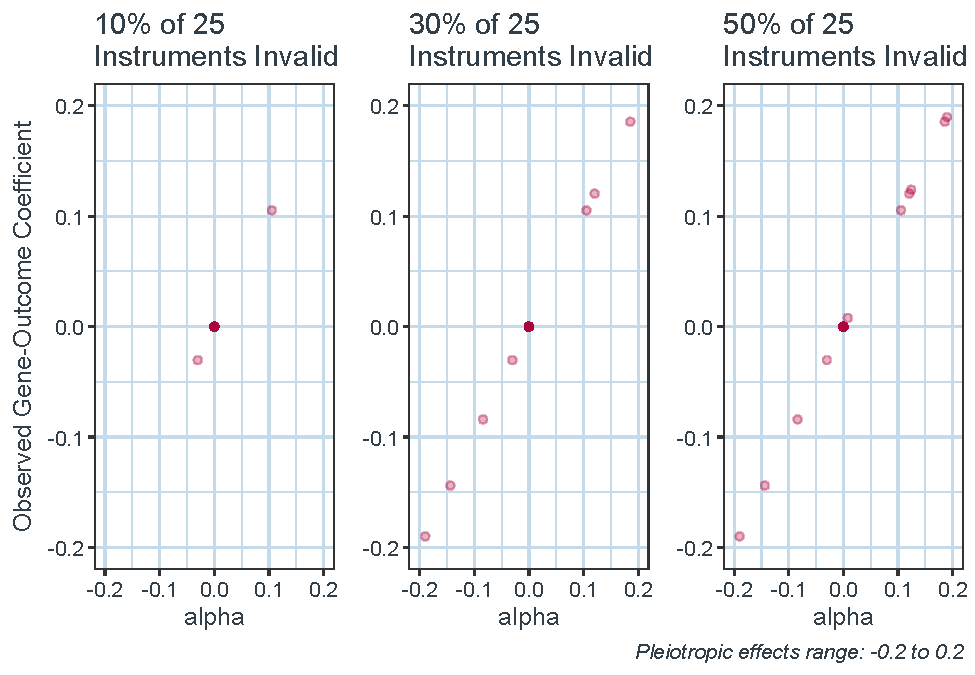
\includegraphics{9_Test_Appendices_files/figure-latex/test-plot-prop-invalid-1.pdf}

Similarly, with random error terms set to 0 and no causal effect present, gene:exposure coefficients estimated for each instrument should exactly match the actual alues simulated, i.e.~\texttt{coeff\_G\_X\ =\ gamma} for all instruments:

\begin{Shaded}
\begin{Highlighting}[]
\CommentTok{\# Check observed gene:exposure coefficients for each instrument}
\CommentTok{\# (coeff\_G\_X) approximate true values (gamma) when a causal effect}
\CommentTok{\# is present \& a large number of participants are included}
 \FunctionTok{set.seed}\NormalTok{(}\DecValTok{1701}\NormalTok{)}
\NormalTok{ sim\_test\_data\_gamma\_1 }\OtherTok{\textless{}{-}} \FunctionTok{simulate\_MR\_data}\NormalTok{(}\AttributeTok{n\_participants =} \DecValTok{100}\NormalTok{,}
                                           \AttributeTok{n\_instruments =} \DecValTok{25}\NormalTok{,}
                                           \AttributeTok{n\_datasets =} \DecValTok{1}\NormalTok{,}
                                           \AttributeTok{prop\_invalid =} \FloatTok{0.1}\NormalTok{,}
                                           \AttributeTok{causal\_effect =} \ConstantTok{FALSE}\NormalTok{,}
                                           \AttributeTok{rand\_error =} \ConstantTok{FALSE}\NormalTok{,}
                                           \AttributeTok{balanced\_pleio =} \ConstantTok{TRUE}\NormalTok{,}
                                           \AttributeTok{InSIDE\_satisfied =} \ConstantTok{TRUE}\NormalTok{)}


\NormalTok{ test\_plot\_tib\_gamma\_1 }\OtherTok{\textless{}{-}} \FunctionTok{extract\_models}\NormalTok{(sim\_test\_data\_gamma\_1)[[}\DecValTok{1}\NormalTok{]]}

\NormalTok{ test\_plot\_tib\_gamma\_1 }\SpecialCharTok{\%\textgreater{}\%}
   \FunctionTok{select}\NormalTok{(gamma, coeff\_G\_X) }\SpecialCharTok{\%\textgreater{}\%}
   \FunctionTok{plot\_template}\NormalTok{() }\SpecialCharTok{+}
   \FunctionTok{geom\_point}\NormalTok{(}\AttributeTok{colour =}\NormalTok{ edin\_bright\_red\_hex, }\AttributeTok{alpha =} \FloatTok{0.3}\NormalTok{) }\SpecialCharTok{+}
   \FunctionTok{aes}\NormalTok{(}\AttributeTok{x =}\NormalTok{ gamma, }\AttributeTok{y =}\NormalTok{ coeff\_G\_X ) }\SpecialCharTok{+}
   \FunctionTok{labs}\NormalTok{(}\AttributeTok{y =} \StringTok{"Observed Gene:Exposure Coefficient"}\NormalTok{,}
        \AttributeTok{title =} \StringTok{"Test: Actual and Estimated Gene:Exposure Coefficients Match"}\NormalTok{)}
\end{Highlighting}
\end{Shaded}

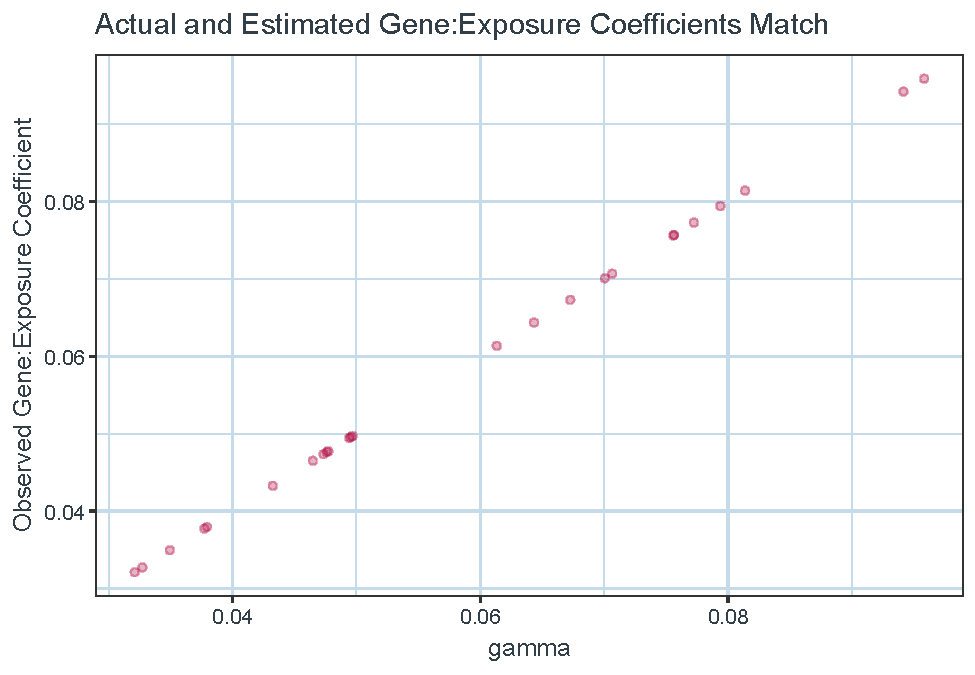
\includegraphics{9_Test_Appendices_files/figure-latex/test-plot-gamma-1-1.pdf}

For the next phase of testing, a function (\texttt{plot\_GY\_GX}) was written to plot the coefficients for gene:exposure versus gene:outcome as estimated using the reviously created linear models:

\begin{Shaded}
\begin{Highlighting}[]
\NormalTok{ plot\_GY\_GX }\OtherTok{\textless{}{-}} \ControlFlowTok{function}\NormalTok{(model\_tib,}
                        \AttributeTok{plot\_title =} \FunctionTok{as.character}\NormalTok{(}\ConstantTok{NA}\NormalTok{),}
                        \AttributeTok{x\_min =} \DecValTok{0}\NormalTok{,                    }\CommentTok{\# set x{-}axis limits}
                        \AttributeTok{x\_max =} \FloatTok{0.1}\NormalTok{,}
                        \AttributeTok{y\_min =} \SpecialCharTok{{-}}\FloatTok{0.05}\NormalTok{,                }\CommentTok{\# set x{-}axis limits}
                        \AttributeTok{y\_max =} \FloatTok{0.06}\NormalTok{,}
                        \AttributeTok{beta\_x =} \FloatTok{0.075}\NormalTok{,               }\CommentTok{\# set beta{-}hat position}
                        \AttributeTok{beta\_y =} \FloatTok{0.05}\NormalTok{,}
                        \AttributeTok{hat\_offset =} \FloatTok{0.003}
\NormalTok{                        )}
\NormalTok{   \{}

\NormalTok{   model\_tib }\SpecialCharTok{\%\textgreater{}\%}
     \FunctionTok{mutate}\NormalTok{(}\AttributeTok{Gradient =} \FunctionTok{round}\NormalTok{(}\FunctionTok{coefficients}\NormalTok{(}\FunctionTok{lm}\NormalTok{(coeff\_G\_Y }\SpecialCharTok{\textasciitilde{}} \DecValTok{0} \SpecialCharTok{+}\NormalTok{ coeff\_G\_X, }\AttributeTok{digits =} \DecValTok{2}\NormalTok{))[}\DecValTok{1}\NormalTok{], }\DecValTok{5}\NormalTok{)) }\SpecialCharTok{\%\textgreater{}\%}
     \FunctionTok{plot\_template}\NormalTok{() }\SpecialCharTok{+}
     \FunctionTok{aes}\NormalTok{(}\AttributeTok{x =}\NormalTok{ coeff\_G\_X, }\AttributeTok{y =}\NormalTok{ coeff\_G\_Y) }\SpecialCharTok{+}
     \FunctionTok{geom\_point}\NormalTok{(}\AttributeTok{colour =}\NormalTok{ edin\_bright\_red\_hex, }\AttributeTok{alpha =} \FloatTok{0.3}\NormalTok{) }\SpecialCharTok{+}
     \FunctionTok{geom\_abline}\NormalTok{(}\FunctionTok{aes}\NormalTok{(}\AttributeTok{intercept =} \DecValTok{0}\NormalTok{,}
                     \AttributeTok{slope =}\NormalTok{ Gradient),}
                 \AttributeTok{size =} \DecValTok{1}\NormalTok{,}
                 \AttributeTok{colour =}\NormalTok{ edin\_uni\_blue\_hex) }\SpecialCharTok{+}
     \FunctionTok{geom\_text}\NormalTok{(}\FunctionTok{aes}\NormalTok{(}\AttributeTok{x =}\NormalTok{ beta\_x,}\CommentTok{\# labels with gradient (causal effect estimate)}
                   \AttributeTok{y =}\NormalTok{ beta\_y,}
                   \AttributeTok{label =} \FunctionTok{paste0}\NormalTok{(}\StringTok{"\textbackslash{}U03B2 == "}\NormalTok{, }\FunctionTok{as.character}\NormalTok{(Gradient))),}\CommentTok{\#beta}
               \AttributeTok{colour =}\NormalTok{ edin\_uni\_blue\_hex,}
               \AttributeTok{hjust =} \DecValTok{0}\NormalTok{,}
               \AttributeTok{parse =} \ConstantTok{TRUE}\NormalTok{) }\SpecialCharTok{+}
     \FunctionTok{annotate}\NormalTok{(}\StringTok{"text"}\NormalTok{,}
              \AttributeTok{x =}\NormalTok{ beta\_x,     }\CommentTok{\# add hat to beta}
              \AttributeTok{y =}\NormalTok{ beta\_y }\SpecialCharTok{+}\NormalTok{ hat\_offset,}
              \AttributeTok{label =} \FunctionTok{paste}\NormalTok{(}\StringTok{"\textbackslash{}U02C6"}\NormalTok{),}
              \AttributeTok{colour =}\NormalTok{ edin\_uni\_blue\_hex,}
              \AttributeTok{hjust =} \SpecialCharTok{{-}}\FloatTok{0.4}\NormalTok{,}
              \AttributeTok{vjust =} \FloatTok{0.9}\NormalTok{,}
              \AttributeTok{parse =} \ConstantTok{TRUE}\NormalTok{) }\SpecialCharTok{+}
     \FunctionTok{labs}\NormalTok{(}\AttributeTok{title =}\NormalTok{ plot\_title,}
          \AttributeTok{x =} \StringTok{"Gene:Exposure Coefficient"}\NormalTok{,}
          \AttributeTok{y =} \StringTok{"Gene:Outcome Coefficient"}\NormalTok{) }\SpecialCharTok{+}
     \FunctionTok{xlim}\NormalTok{(x\_min, x\_max) }\SpecialCharTok{+}
     \FunctionTok{ylim}\NormalTok{(y\_min, y\_max)}

\NormalTok{ \}}
\end{Highlighting}
\end{Shaded}

\begin{Shaded}
\begin{Highlighting}[]
\CommentTok{\# No causal effect present}
 \FunctionTok{set.seed}\NormalTok{(}\DecValTok{1701}\NormalTok{)}
\NormalTok{ sim\_test\_data\_causal\_0 }\OtherTok{\textless{}{-}} \FunctionTok{simulate\_MR\_data}\NormalTok{(}\AttributeTok{n\_participants =} \DecValTok{1000}\NormalTok{,}
                                            \AttributeTok{n\_instruments =} \DecValTok{100}\NormalTok{,}
                                            \AttributeTok{n\_datasets =} \DecValTok{1}\NormalTok{,}
                                            \AttributeTok{prop\_invalid =} \DecValTok{0}\NormalTok{,}
                                            \AttributeTok{causal\_effect =} \ConstantTok{FALSE}\NormalTok{,}
                                            \AttributeTok{rand\_error =} \ConstantTok{FALSE}\NormalTok{)}

\NormalTok{ test\_plot\_tib\_causal\_0 }\OtherTok{\textless{}{-}} \FunctionTok{extract\_models}\NormalTok{(sim\_test\_data\_causal\_0)[[}\DecValTok{1}\NormalTok{]]}

 \FunctionTok{plot\_GY\_GX}\NormalTok{(test\_plot\_tib\_causal\_0, }\AttributeTok{plot\_title =} \StringTok{"No Causal Effect"}\NormalTok{)}
\end{Highlighting}
\end{Shaded}

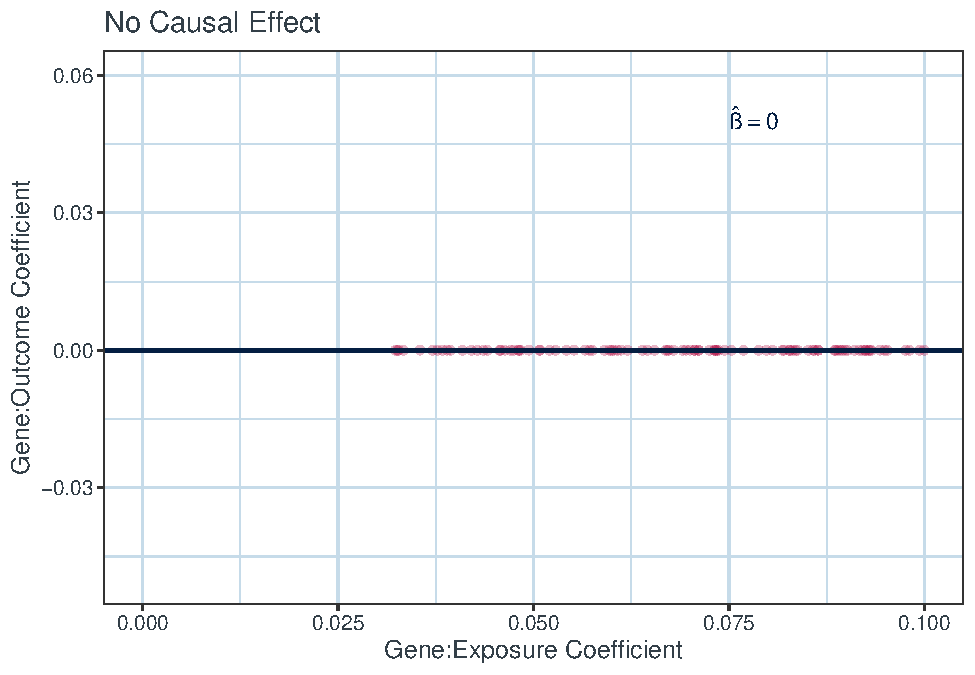
\includegraphics{9_Test_Appendices_files/figure-latex/test-plot-no-causal-1.pdf}

\begin{Shaded}
\begin{Highlighting}[]
\CommentTok{\# Check altering proportion of invalid instruments alters}
\CommentTok{\# proportion of instruments displaying pleiotropic effects}
\CommentTok{\# N.B. cluster around alpha = 0 represents valid instruments with}
\CommentTok{\# no pleiotropic effects}


\CommentTok{\# Causal effect present}
 \FunctionTok{set.seed}\NormalTok{(}\DecValTok{1701}\NormalTok{)}
\NormalTok{ sim\_test\_data\_causal\_1 }\OtherTok{\textless{}{-}} \FunctionTok{simulate\_MR\_data}\NormalTok{(}\AttributeTok{n\_participants =} \DecValTok{1000}\NormalTok{,}
                                            \AttributeTok{n\_instruments =} \DecValTok{100}\NormalTok{,}
                                            \AttributeTok{n\_datasets =} \DecValTok{1}\NormalTok{,}
                                            \AttributeTok{prop\_invalid =} \DecValTok{0}\NormalTok{,}
                                            \AttributeTok{causal\_effect =} \ConstantTok{TRUE}\NormalTok{,}
                                            \AttributeTok{rand\_error =} \ConstantTok{FALSE}\NormalTok{,}
                                            \AttributeTok{two\_sample =} \ConstantTok{FALSE}\NormalTok{)}

\NormalTok{ test\_plot\_tib\_causal\_1 }\OtherTok{\textless{}{-}} \FunctionTok{extract\_models}\NormalTok{(sim\_test\_data\_causal\_1)[[}\DecValTok{1}\NormalTok{]]}

 \FunctionTok{plot\_GY\_GX}\NormalTok{(test\_plot\_tib\_causal\_1, }\AttributeTok{plot\_title =} \StringTok{"Causal Effect Present"}\NormalTok{)}
\end{Highlighting}
\end{Shaded}

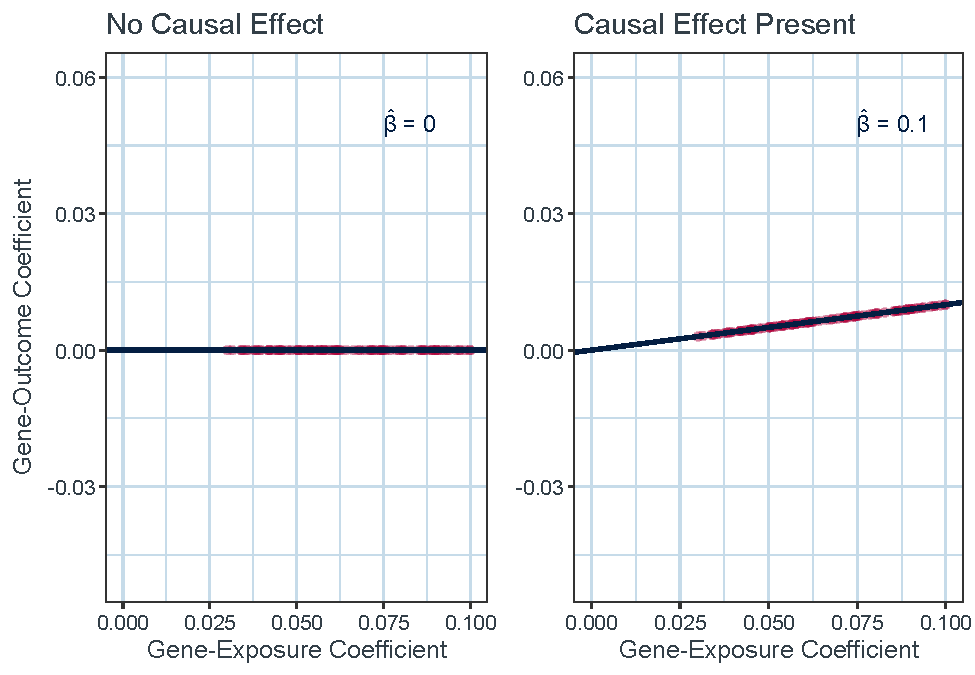
\includegraphics{9_Test_Appendices_files/figure-latex/test-plot-causal-1.pdf}

\begin{Shaded}
\begin{Highlighting}[]
\CommentTok{\# Check violating InSIDE assumption results in distorted}
\CommentTok{\# estimation of pleiotropic effects}
\CommentTok{\# N.B. cluster around alpha = 0 represents valid instruments with}
\CommentTok{\# no pleiotropic effects}
 \FunctionTok{set.seed}\NormalTok{(}\DecValTok{1701}\NormalTok{)}
\NormalTok{ sim\_test\_data\_phi\_T }\OtherTok{\textless{}{-}} \FunctionTok{simulate\_MR\_data}\NormalTok{(}\AttributeTok{n\_participants =} \DecValTok{100000}\NormalTok{,}
                                         \AttributeTok{n\_instruments =} \DecValTok{100}\NormalTok{,}
                                         \AttributeTok{n\_datasets =} \DecValTok{1}\NormalTok{,}
                                         \AttributeTok{prop\_invalid =} \FloatTok{0.3}\NormalTok{,}
                                         \AttributeTok{causal\_effect =} \ConstantTok{FALSE}\NormalTok{,}
                                         \AttributeTok{balanced\_pleio =} \ConstantTok{FALSE}\NormalTok{,}
                                         \AttributeTok{InSIDE\_satisfied =} \ConstantTok{FALSE}\NormalTok{)}

 \FunctionTok{set.seed}\NormalTok{(}\DecValTok{1701}\NormalTok{)}
\NormalTok{ sim\_test\_data\_phi\_F }\OtherTok{\textless{}{-}} \FunctionTok{simulate\_MR\_data}\NormalTok{(}\AttributeTok{n\_participants =} \DecValTok{100000}\NormalTok{,}
                                         \AttributeTok{n\_instruments =} \DecValTok{100}\NormalTok{,}
                                         \AttributeTok{n\_datasets =} \DecValTok{1}\NormalTok{,}
                                         \AttributeTok{prop\_invalid =} \FloatTok{0.3}\NormalTok{,}
                                         \AttributeTok{causal\_effect =} \ConstantTok{FALSE}\NormalTok{,}
                                         \AttributeTok{balanced\_pleio =} \ConstantTok{FALSE}\NormalTok{,}
                                         \AttributeTok{InSIDE\_satisfied =} \ConstantTok{TRUE}\NormalTok{)}


\NormalTok{ test\_plot\_tib\_phi\_T }\OtherTok{\textless{}{-}} \FunctionTok{extract\_models}\NormalTok{(sim\_test\_data\_phi\_T)[[}\DecValTok{1}\NormalTok{]]}
\NormalTok{ test\_plot\_tib\_phi\_F }\OtherTok{\textless{}{-}} \FunctionTok{extract\_models}\NormalTok{(sim\_test\_data\_phi\_F)[[}\DecValTok{1}\NormalTok{]]}

\NormalTok{ test\_plot\_tib\_phi\_T }\SpecialCharTok{\%\textgreater{}\%}
   \FunctionTok{select}\NormalTok{(phi, coeff\_G\_Y) }\SpecialCharTok{\%\textgreater{}\%}
   \FunctionTok{plot}\NormalTok{(.,}
        \AttributeTok{main =} \StringTok{"InSIDE Violated"}\NormalTok{,}
        \AttributeTok{ylab =} \StringTok{"Gene:Outcome Coefficient"}\NormalTok{)}
\end{Highlighting}
\end{Shaded}

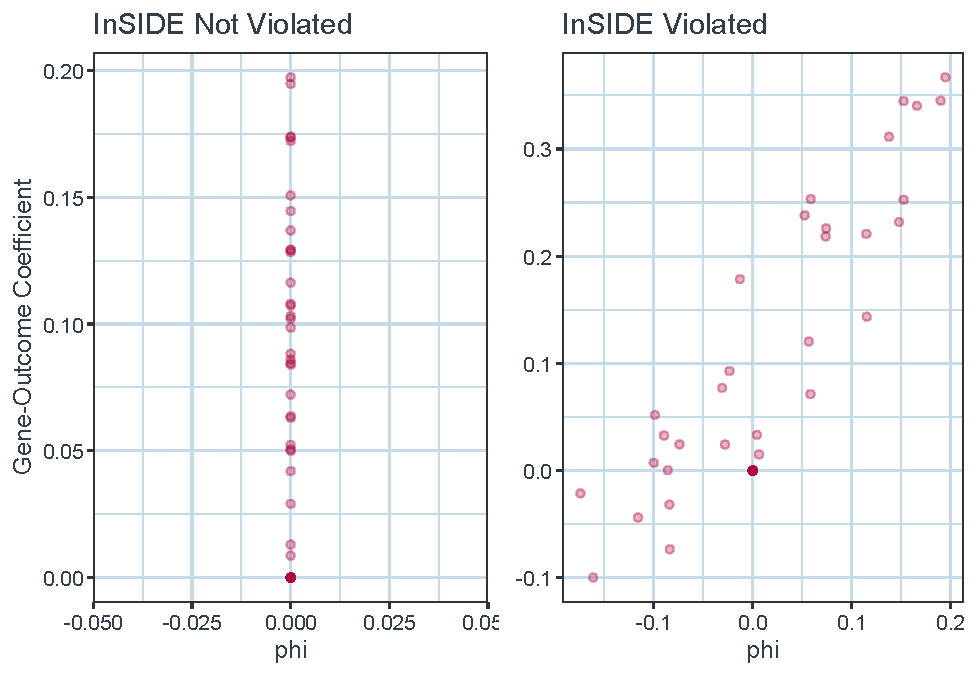
\includegraphics{9_Test_Appendices_files/figure-latex/test-plot-phi-2-1.pdf}

\begin{Shaded}
\begin{Highlighting}[]
\NormalTok{ test\_plot\_tib\_phi\_F }\SpecialCharTok{\%\textgreater{}\%}
   \FunctionTok{select}\NormalTok{(phi, coeff\_G\_Y) }\SpecialCharTok{\%\textgreater{}\%}
   \FunctionTok{plot}\NormalTok{(.,}
        \AttributeTok{main =} \StringTok{"InSIDE Not Violated"}\NormalTok{,}
        \AttributeTok{ylab =} \StringTok{"Gene:Outcome Coefficient"}\NormalTok{)}
\end{Highlighting}
\end{Shaded}

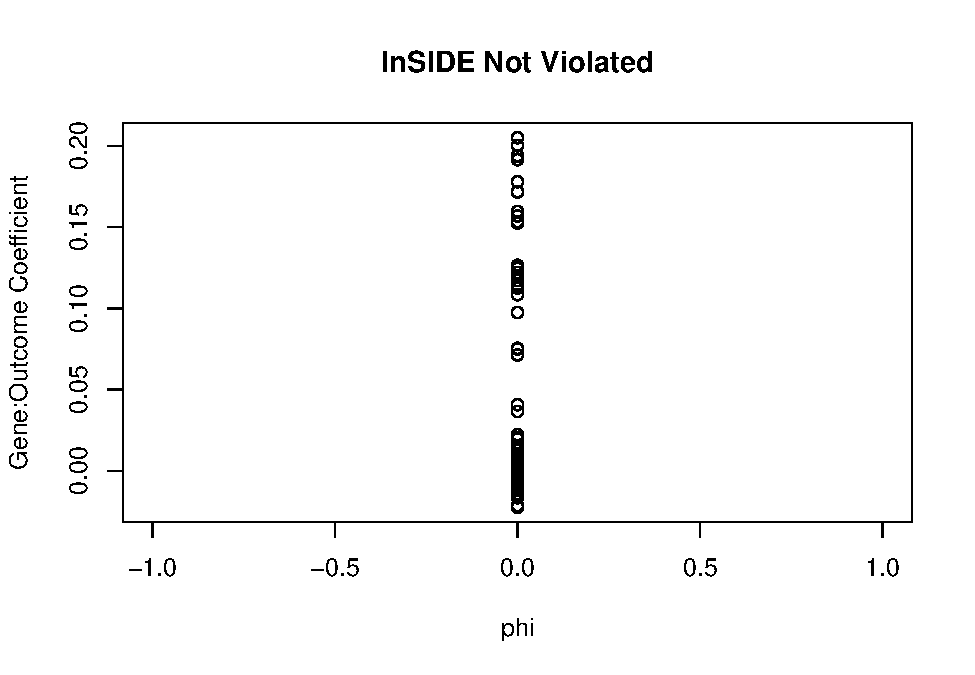
\includegraphics{9_Test_Appendices_files/figure-latex/test-plot-phi-2-2.pdf}

\begin{Shaded}
\begin{Highlighting}[]
\CommentTok{\#phi on y, not alpha}
\end{Highlighting}
\end{Shaded}

\newpage

\subsection{Appendix C: Citation Search Strategy}\label{appendix-c-citation-search-strategy}

\end{document}
